\documentclass{amsart}
\usepackage{graphicx}
\vfuzz2pt % Don't report over-full v-boxes if over-edge is small
\hfuzz2pt % Don't report over-full h-boxes if over-edge is small
\newtheorem{thm}{Theorem}[section]
\newtheorem{cor}[thm]{images/Corollary}
\newtheorem{lem}[thm]{images/Lemma}
\newtheorem{prop}[thm]{images/Proposition}
\theoremstyle{definition}
\newtheorem{defn}[thm]{images/Definition}
\theoremstyle{remark}
\newtheorem{rem}[thm]{images/Remark}
\numberwithin{equation}{section}
\newcommand{\norm}[1]{images/\left\Vert#1\right\Vert}
\newcommand{\abs}[1]{images/\left\vert#1\right\vert}
\newcommand{\set}[1]{images/\left\{#1\right\}}
\newcommand{\Real}{\mathbb R}
\newcommand{\eps}{\varepsilon}
\newcommand{\To}{\longrightarrow}
\newcommand{\BX}{\mathbf{B}(X)}
\newcommand{\A}{\mathcal{A}}
\begin{document}
\title{Digital Color Reproduction : Notes and Definitions }
\author{Bruce Campbell}%
\address{}%
\email{wavescholar@gmail.com}%
\thanks{The author would like to acknowledge the support of his teammates : Andre Henry, Matt Trevors, Quinten Mercer III, Tyke Czekalski}%
\begin{abstract}
Notes and definitions on color reproduction
\end{abstract}
\maketitle
\section{Definitions and Concepts}
Color Science concerns itself with the characterization of perception of color stimuli, the synthesis of stimuli from perception, and the processing of color information.  Characterization of perceptions from stimuli involves measurement and descriptive processes.  Color reproduction and processing form the basis of most digital applications of color science with the aim to provide a stimulus giving rise to a target perception.  Tristimulus colorimetry is based on three color matching functions which define the primary colors which are mixed to produce a range of stimuli.  The perception of an isolated stimulus is matched to an additive mixture of three light sources called primaries $R, G, B$.  The perception induced by a stimulus is characterized by three values $X, Y, Z$ related to the luminance of the primaries.  Linearly independent light sources are used to create a color measurement system where the tristimulus values encode the amount of each primary required to reproduce a color stimuli.  To calculate a tristimulus value we integrate the spectral distribution of the light source $\phi(\lambda)$ multiplied by the color matching function

\begin{eqnarray*}
\nonumber
  X &=& \int R(\lambda) \phi(\lambda) d\lambda  \\
  Y &=& \int G(\lambda) \phi(\lambda) d\lambda \\
  Z &=& \int B(\lambda) \phi(\lambda) d\lambda
\end{eqnarray*}

\begin{figure}
  \caption{Spectra of CIE Daylight and Fluorescent Illuminants}
  \begin{center}
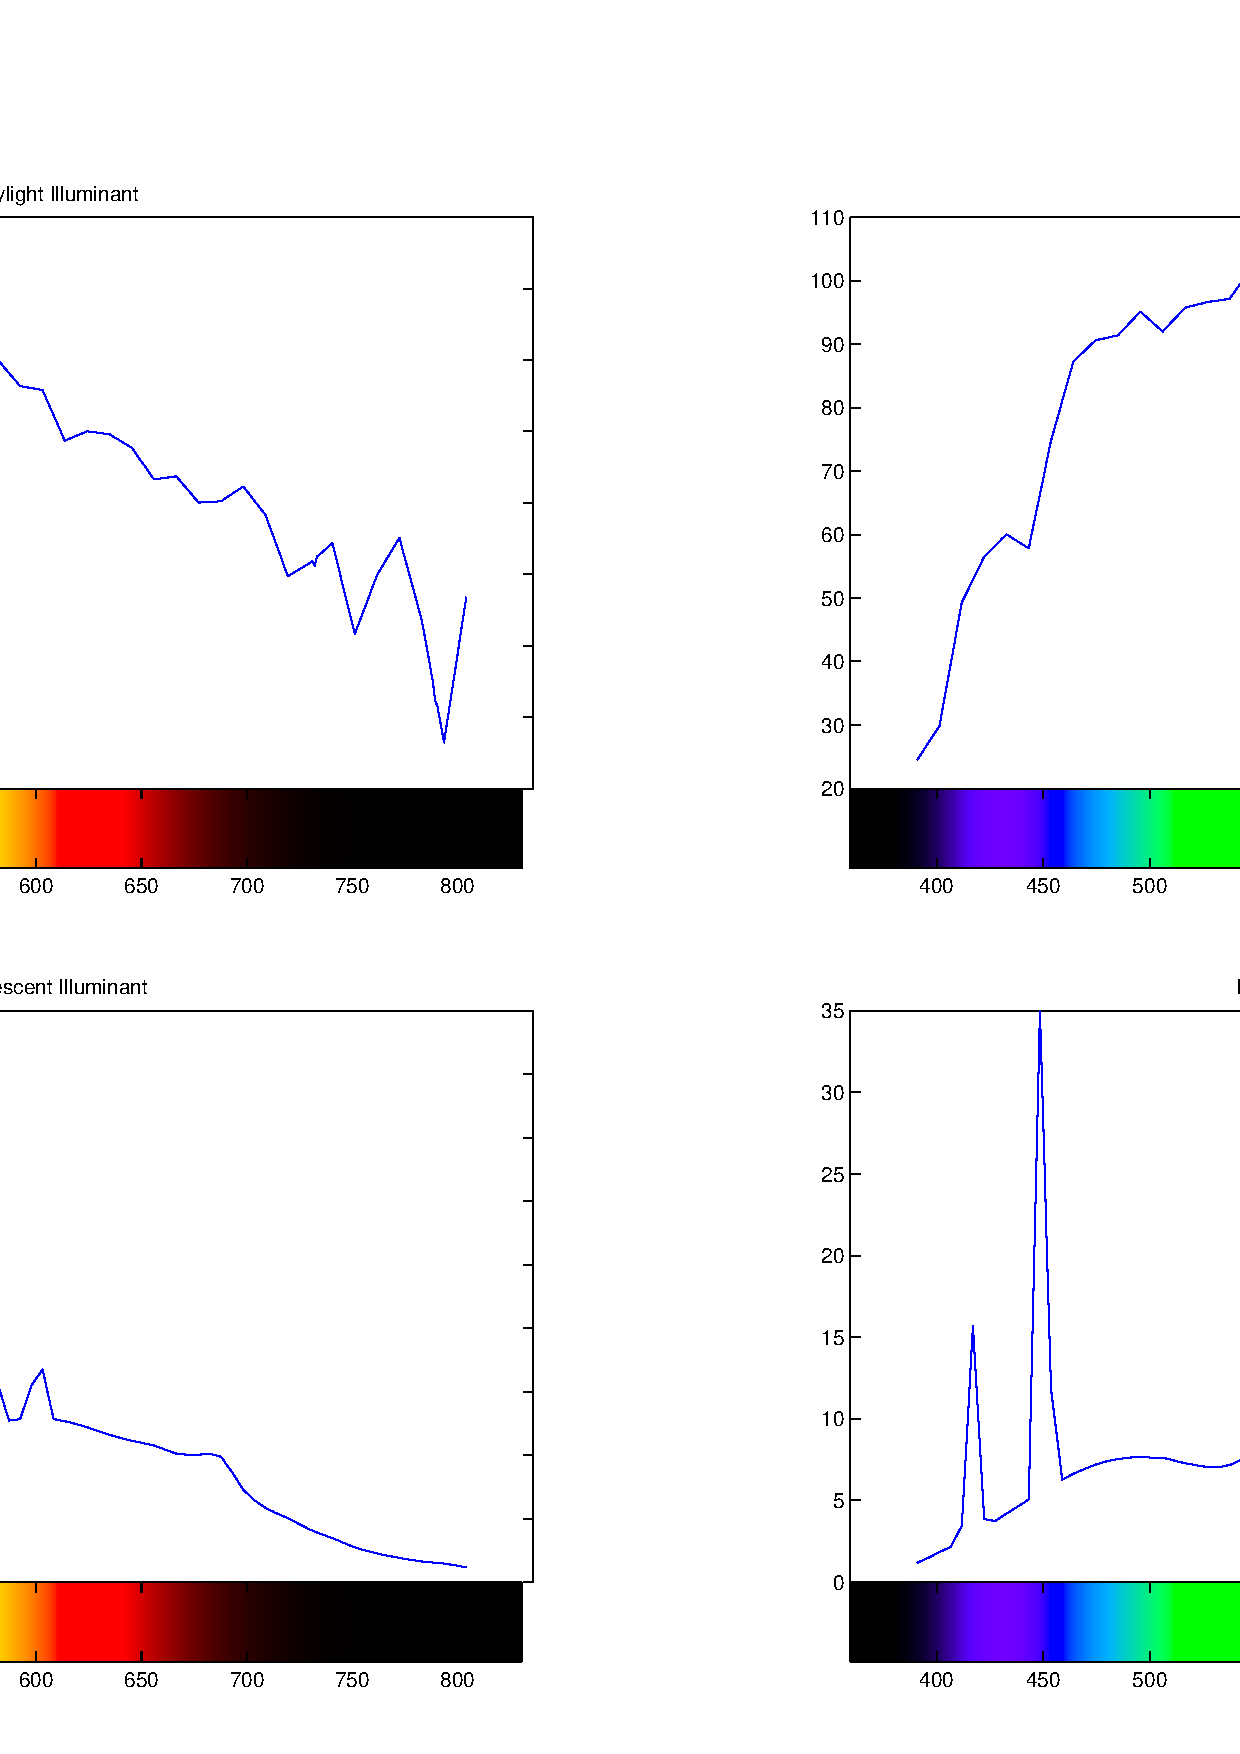
\includegraphics[width=12.0cm]{images/daylight_Flourcescent.jpg}
  \end{center}
\end{figure}

\begin{figure}
  \caption{Color Matching Functions for CIE Standard Observer}
  \begin{center}
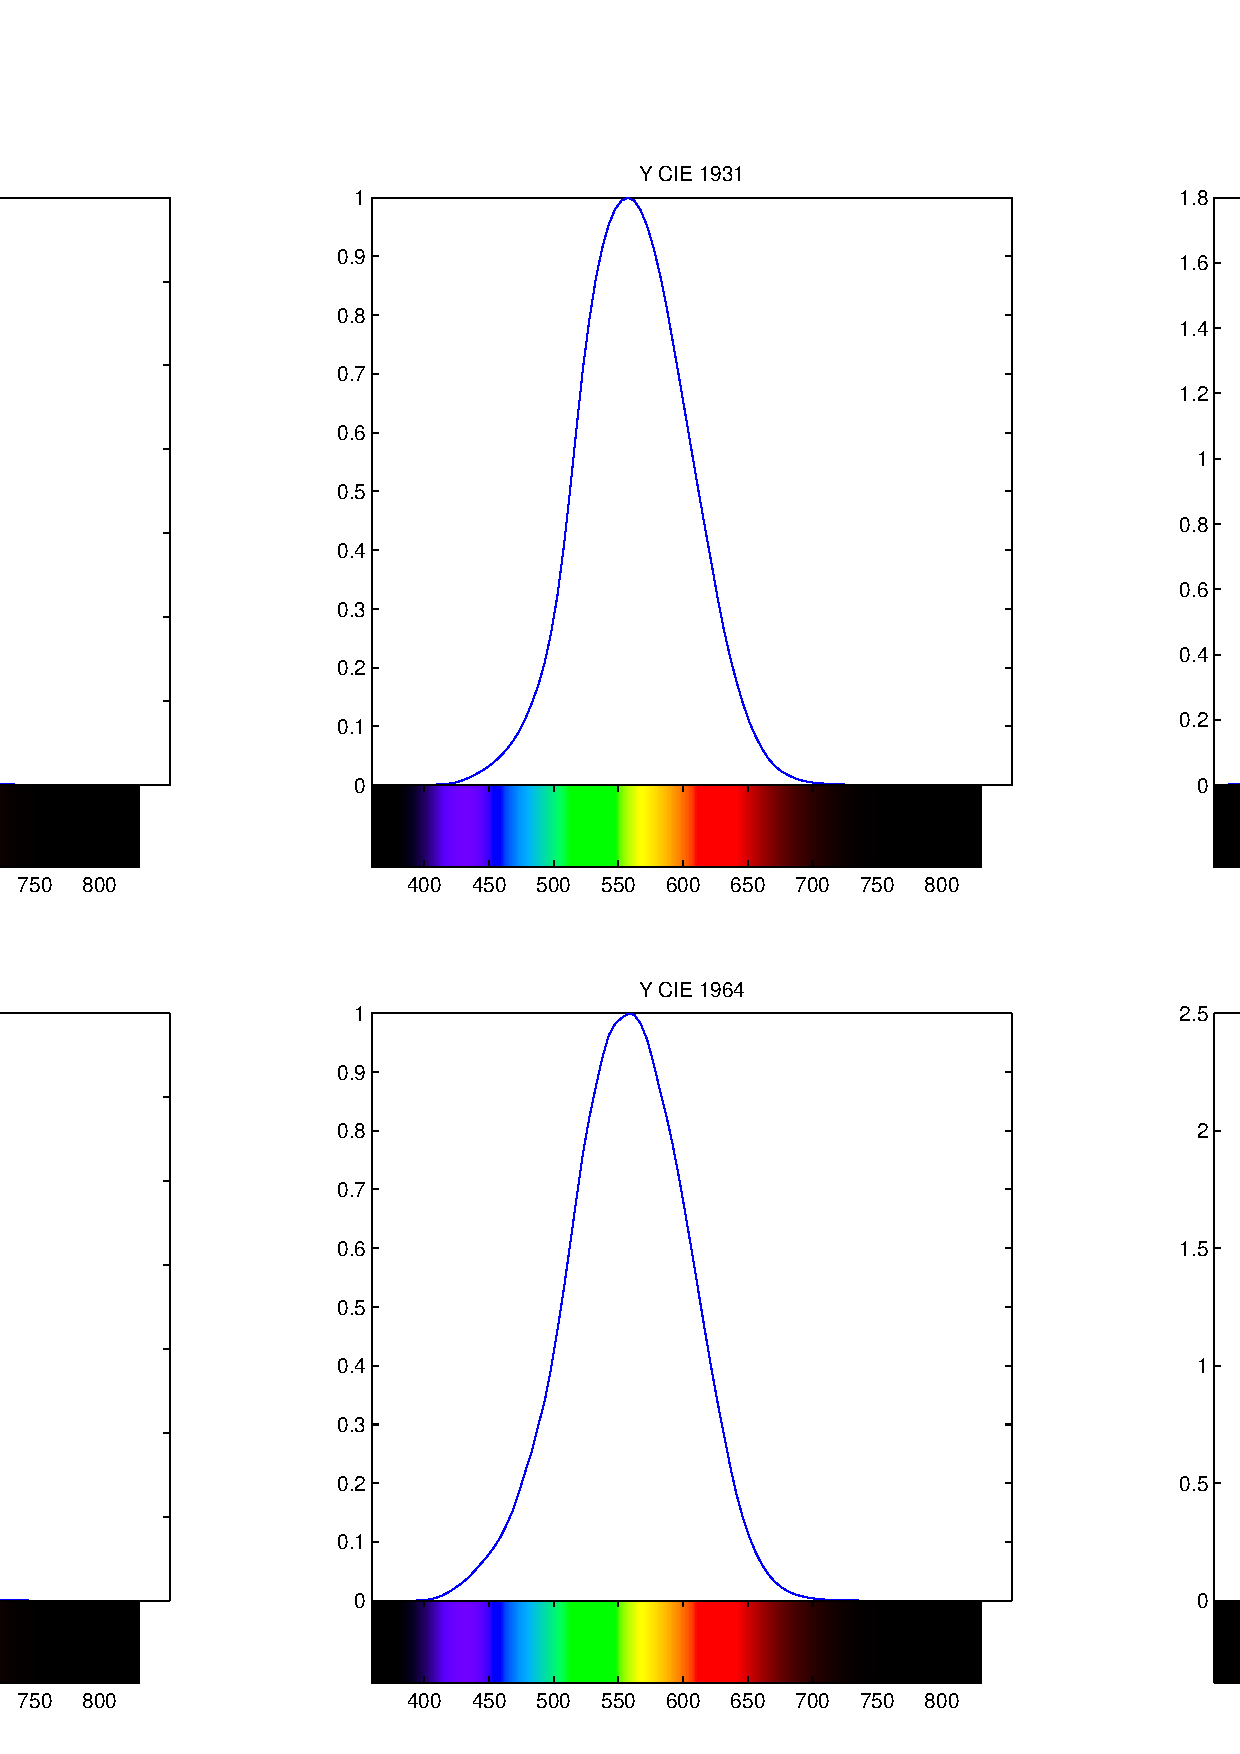
\includegraphics[width=12.0cm]{images/XYZ_CMF.jpg}
  \end{center}
\end{figure}
Tristimulus values relate the radiance from a stimulus to the color matching functions.  For color reproduction a set of primaries are fixed and the  tristimulus vector in that color space provides luminances of the primaries required to generate the stimuli.  Color processing is any modification of the color content of a digital image. In order to make the processing task intuitive it has to be done in a representation correlated with the perceptual dimensions of color.  $X, Y, Z$ tristimulus values are not uniform when describing differences in colors.  The CIE Lab color space is a non-linear transform of tristimulus values to a perceptually uniform color space. The transform from tristimulus values to Lab was designed to reproduce the response of the human eye. CIE Lab describes all the colors visible to the human visual system and serves as a device independent color model.  Uniform changes in the Lab color space correspond to uniform changes in color perception.

Chromaticity is an specification of the quality of a color regardless of its luminance. In the Lab color space this is an easy projection on to the ab-plane. The white point of an illuminant is a neutral reference point in the ab-plane.

An absolute color space is one in which which the perceptual difference between colors relates to distances between colors as represented by points in the color space.  Another common definition of an absolute color space is one in which the colors characterized without having to specify an illuminant.
CIEXYZ and sRGB are absolute color spaces. CIE Lab is absolute if one specifies the white point.
There are no simple formulas for conversion between raw RGB values and Lab without the use of an ICC profile or specification of the spectral properties of the primaries and the illuminant.
Converting between non-absolute color spaces or between absolute and non-absolute color spaces has no visual meaning.

An absolute color space can be reversibly converted into another absolute color space but gamut limitations may prevent all of the colors from making the round trip.  Gamut mapping algorithms are typically tuned to preserve application sensitive colors or to minimize overall error.

\subsection{Reflective and Transmissive Models of Color Perception}
The spectral reflectance values obtained from a Macbeth Color chart. 

\begin{tabular}{  c c c c }
\includegraphics[width=3.0cm,height=3.0cm]{images/ch1.jpg}
&
\includegraphics[width=3.0cm,height=3.0cm]{images/ch2.jpg}
&
\includegraphics[width=3.0cm,height=3.0cm]{images/ch3.jpg}
&
\includegraphics[width=3.0cm,height=3.0cm]{images/ch4.jpg}
\\

\includegraphics[width=3.0cm,height=3.0cm]{images/ch5.jpg}
&
\includegraphics[width=3.0cm,height=3.0cm]{images/ch6.jpg}
&
\includegraphics[width=3.0cm,height=3.0cm]{images/ch7.jpg}
&
\includegraphics[width=3.0cm,height=3.0cm]{images/ch8.jpg}
\\

\includegraphics[width=3.0cm,height=3.0cm]{images/ch9.jpg}
&
\includegraphics[width=3.0cm,height=3.0cm]{images/ch10.jpg}
&
\includegraphics[width=3.0cm,height=3.0cm]{images/ch11.jpg}
&
\includegraphics[width=3.0cm,height=3.0cm]{images/ch12.jpg}
\\

\includegraphics[width=3.0cm,height=3.0cm]{images/ch13.jpg}
&
\includegraphics[width=3.0cm,height=3.0cm]{images/ch14.jpg}
&
\includegraphics[width=3.0cm,height=3.0cm]{images/ch15.jpg}
&
\includegraphics[width=3.0cm,height=3.0cm]{images/ch16.jpg}
\\

\includegraphics[width=3.0cm,height=3.0cm]{images/ch17.jpg}
&
\includegraphics[width=3.0cm,height=3.0cm]{images/ch18.jpg}
&
\includegraphics[width=3.0cm,height=3.0cm]{images/ch19.jpg}
&
\includegraphics[width=3.0cm,height=3.0cm]{images/ch20.jpg}
\\

\includegraphics[width=3.0cm,height=3.0cm]{images/ch21.jpg}
&
\includegraphics[width=3.0cm,height=3.0cm]{images/ch22.jpg}
&
\includegraphics[width=3.0cm,height=3.0cm]{images/ch23.jpg}
&
\includegraphics[width=3.0cm,height=3.0cm]{images/ch24.jpg}
\end{tabular}

\subsection{Additive and Subtractive Color Models}

\subsection{Gamut Mapping}
Definition definitions used by the CIE TC 8-03 on gamut mapping are given below.

Image: two-dimensional stimulus containing pictorial or graphical information whereby the original
image is the image to which its reproductions are compared in terms of some characteristics.

Color reproduction medium: a medium for displaying or capturing color information, e.g. a CRT
monitor, a digital camera or a scanner. Note that in the case of slide scanning, the color reproduction
medium is not the scanner but the combination of scanner, stains and glass substrate.

Color gamut: a range of colors achievable on a given color reproduction medium under a given set of viewing conditions.

Color gamut boundary: a surface determined by a color gamut's extremes.

Gamut boundary descriptor: an overall way of approximately describing a gamut boundary.
Line gamut boundary: the points of intersections between a gamut boundary and a given line along which mapping is to be carried out.

Color gamut mapping: a method for assigning colors from the reproduction medium to colors from the
original medium or image.

Color reproduction intent: the desired relationship between color information in original and
reproduction media. As a number of solutions to cross-media reproduction intents can be pursued by
gamut mapping. The most generic of these are accuracy and pleasantness but it is also possible to
define others for specific application (e.g. to provide an accurate reproduction of corporate
identity colors while giving pleasant results for others). Note that reproduction intents are also
referred to as rendering intents.

Accurate reproduction intent: aims to maximize the degree of similarity between the original image
and a reproduction of it as far as possible, given the constraints of the color reproduction media
involved. Note that the characteristic of accurate reproduction is intrinsically relative (i.e.
reproduction versus original).

Pleasant reproduction intent: aims to maximize the reproduction's correspondence with preconceived
ideas of given image should look according to an individual whereby this criterion encompasses
contrast, lack of artifacts, sharpness, etc. Note that unlike accuracy, pleasantness is absolute at
least as far as given observer understands it at a given moment.

The images below display various perspectives of the gamut of a scanner device [solid] and the sRGB color space [wire].

\includegraphics[width=5.0cm]{images/aperio_sRGB_v1.jpg}

\includegraphics[width=5.0cm]{images/aperio_sRGB_v2.jpg}

\includegraphics[width=5.0cm]{images/aperio_sRGB_v3.jpg}

\includegraphics[width=5.0cm]{images/aperio_sRGB_v4.jpg}

\subsection{Rendering Intents}
There are 4 rendering intents defined by the International Color Consortium (ICC), which are
specifically defined for the purposes of cross media reproduction using color management
systems. The intents are related to the gamut mapping techniques.

Perceptual intent: the full gamut is compressed to fill the gamut of the destination
device. Gray balance is preserved, the relationship between the colors is not altered
but colorimetric accuracy might not be preserved, as all the colors are moved.
Saturation intent: it converts the saturated colors in the source gamut to the saturated
colors in the destination gamut. This transformation is done at the expense of
accuracy in hue and lightness.

Relative colorimetric intent: only the colors that are outside the destination gamut are
clipped to the destination gamut boundaries. It may result that two different colors of
the source gamut are mapped into the same color in the destination profile. The
relative colorimetric intent takes into account the fact that our eyes always adapt to the white of a medium. The white on the output is the white of the medium and not the
white of the source profile.

Absolute colorimetric intent: it is similar to the relative colorimetric intent except that
the white point of the source and destination are the same. This mode is used for
proofing, where we want to simulate the output of one printer to another device.

\subsection{Affine Transforms of RAW RGB values}
There are a number of non-absolute color transformations that are used in image processing for convenience.  Compression rates in the encoding of JPEG and JPEG 2000 are increased when the RGB values are converted to YCbCr by an affine transform of the RGB values that places most of the color information in the second two components.
These types of transforms are reversible except for floating point roundoff errors.
%\begin{figure}
%  \caption{RGB Cube Transformed to YCbCr}
%  \begin{center}
\includegraphics[width=12.0cm]{images/RGB_TO_YCBCR.jpg}
%  \end{center}
%\end{figure}

\subsection{Non-Linear Transforms of RAW RGB values}
Color transforms that combine a gamma correction with a rotation of color values are faster that a full gamut mapping transform. The goal of a gamma correction is to obtain an accurate tone scale reproduction.  The associated rotation is usually performed to move luminance data to one channel so that a the non-linear operation takes place in 1 dimension.

\end{document}
